%	This is written by Zhiyang Ong to record notes about bioinformatics of his digital biology class.

%	The MIT License (MIT)

%	Copyright (c) <2014> <Zhiyang Ong>

%	Permission is hereby granted, free of charge, to any person obtaining a copy of this software and associated documentation files (the "Software"), to deal in the Software without restriction, including without limitation the rights to use, copy, modify, merge, publish, distribute, sublicense, and/or sell copies of the Software, and to permit persons to whom the Software is furnished to do so, subject to the following conditions:

%	The above copyright notice and this permission notice shall be included in all copies or substantial portions of the Software.

%	THE SOFTWARE IS PROVIDED "AS IS", WITHOUT WARRANTY OF ANY KIND, EXPRESS OR IMPLIED, INCLUDING BUT NOT LIMITED TO THE WARRANTIES OF MERCHANTABILITY, FITNESS FOR A PARTICULAR PURPOSE AND NONINFRINGEMENT. IN NO EVENT SHALL THE AUTHORS OR COPYRIGHT HOLDERS BE LIABLE FOR ANY CLAIM, DAMAGES OR OTHER LIABILITY, WHETHER IN AN ACTION OF CONTRACT, TORT OR OTHERWISE, ARISING FROM, OUT OF OR IN CONNECTION WITH THE SOFTWARE OR THE USE OR OTHER DEALINGS IN THE SOFTWARE.

%	Email address: echo "cukj -wb- 23wU4X5M589 TROJANS cqkH wiuz2y 0f Mw Stanford" | awk '{ sub("23wU4X5M589","F.d_c_b. ") sub("Stanford","d0mA1n"); print $5, $2, $8; for (i=1; i<=1; i++) print "6\b"; print $9, $7, $6 }' | sed y/kqcbuHwM62z/gnotrzadqmC/ | tr 'q' ' ' | tr -d [:cntrl:] | tr -d 'ir' | tr y "\n" Bioinformatics + Computational Genomics/Genetics

%%%%%%%%%%%%%%%%%%%%%%%%%%%%%%%%%%%%%%%%%%%%%%





%%%%%%%%%%%%%%%%%%%%%%%%%%%%%%%%%%%%%%%%%%%%%%
\chapter{Bioinformatics: Computational Genomics/Genetics}
\label{chp:Administration}

This is a chapter about bioinformatics (particularly computational genomics/genetics). \\

At the end of the class, I should be able to use {\tt Bowtie} (or a comparable bioinformatics tool) to create my own {\tt Bowtie} index/directory for read alignment, when it aligns short DNA sequences (reads) to the human genome.


%%%%%%%%%%%%%%%%%%%%%%%%%%%%%%%%%%%%%%%%%%%%%%
\section{Introductory Bioinformatics}
\label{sec:IntroductoryBioinformatics}





%%%%%%%%%%%%%%%%%%%%%%%%%%%%%%%%%%%%%%%%%%%%%%
\subsection{Advice Regarding Bioinformatics}
\label{ssec:BioinformaticsAdvice}

Some advice regarding bioinformatics are: \vspace{-0.3cm}
\begin{enumerate} \itemsep -4pt
\item When doing a lot of mapping (e.g., genome mapping and transcriptome mapping), put aliases to all datasets in a directory. Don't make multiple copies of files/directories. This redundancy takes up a lot of storage space on the hard disks/drives. When operations/processes are carried out on these copies, they will bog/slow down the computer network. 
\end{enumerate}




%%%%%%%%%%%%%%%%%%%%%%%%%%%%%%%%%%%%%%%%%%%%%%
\section{Bowtie}
\label{sec:Bowtie}

{\tt Bowtie} is a software application for sequence analysis that reads short reads from a DNA/genomic sequence \cite{Langmead2014}.


Some flags for {\tt Bowtie} (Version 1) are discussed as follows: \vspace{-0.3cm}
\begin{enumerate} \itemsep -4pt
\item -v0. Do not allow any misalignment errors.
\item -m1. Do not report multiple ($> 1$) misalignment errors. \vspace{-0.3cm}
	\begin{enumerate} \itemsep -2pt
	\item Therefore, {\tt -m100} does not report $> 100$ misalignment errors. Reads can map between 0 to 100 times, but not more than 100 times (1--100 times), such as 1X, 3X, 49X, or 100X. That is, it suppresses reads that maps to $> 100$ times. It does not demand exact mismatches.
	\item It does strictly not depend on the length of the reads (the size of the mapping, or mapping size).
	\end{enumerate}
\item {\tt -n} versus {\tt -v} is about global versus local alignment: \vspace{-0.3cm}
	\begin{enumerate} \itemsep -2pt
	\item Regarding global alignment, one sequence is matched with another.
	\item As for local alignment, compare one region of a sequence to another region.
	\item Local alignments are more sensitive than global alignments.
	\item Local alignments are less informative than global alignments.
	\end{enumerate}
\item {\tt -v1 -m1} $\rightarrow$ {\tt -v1 -m100} increases the number of reads by a small amount.
\item 
\end{enumerate}

\begin{figure}[h]
\centering 
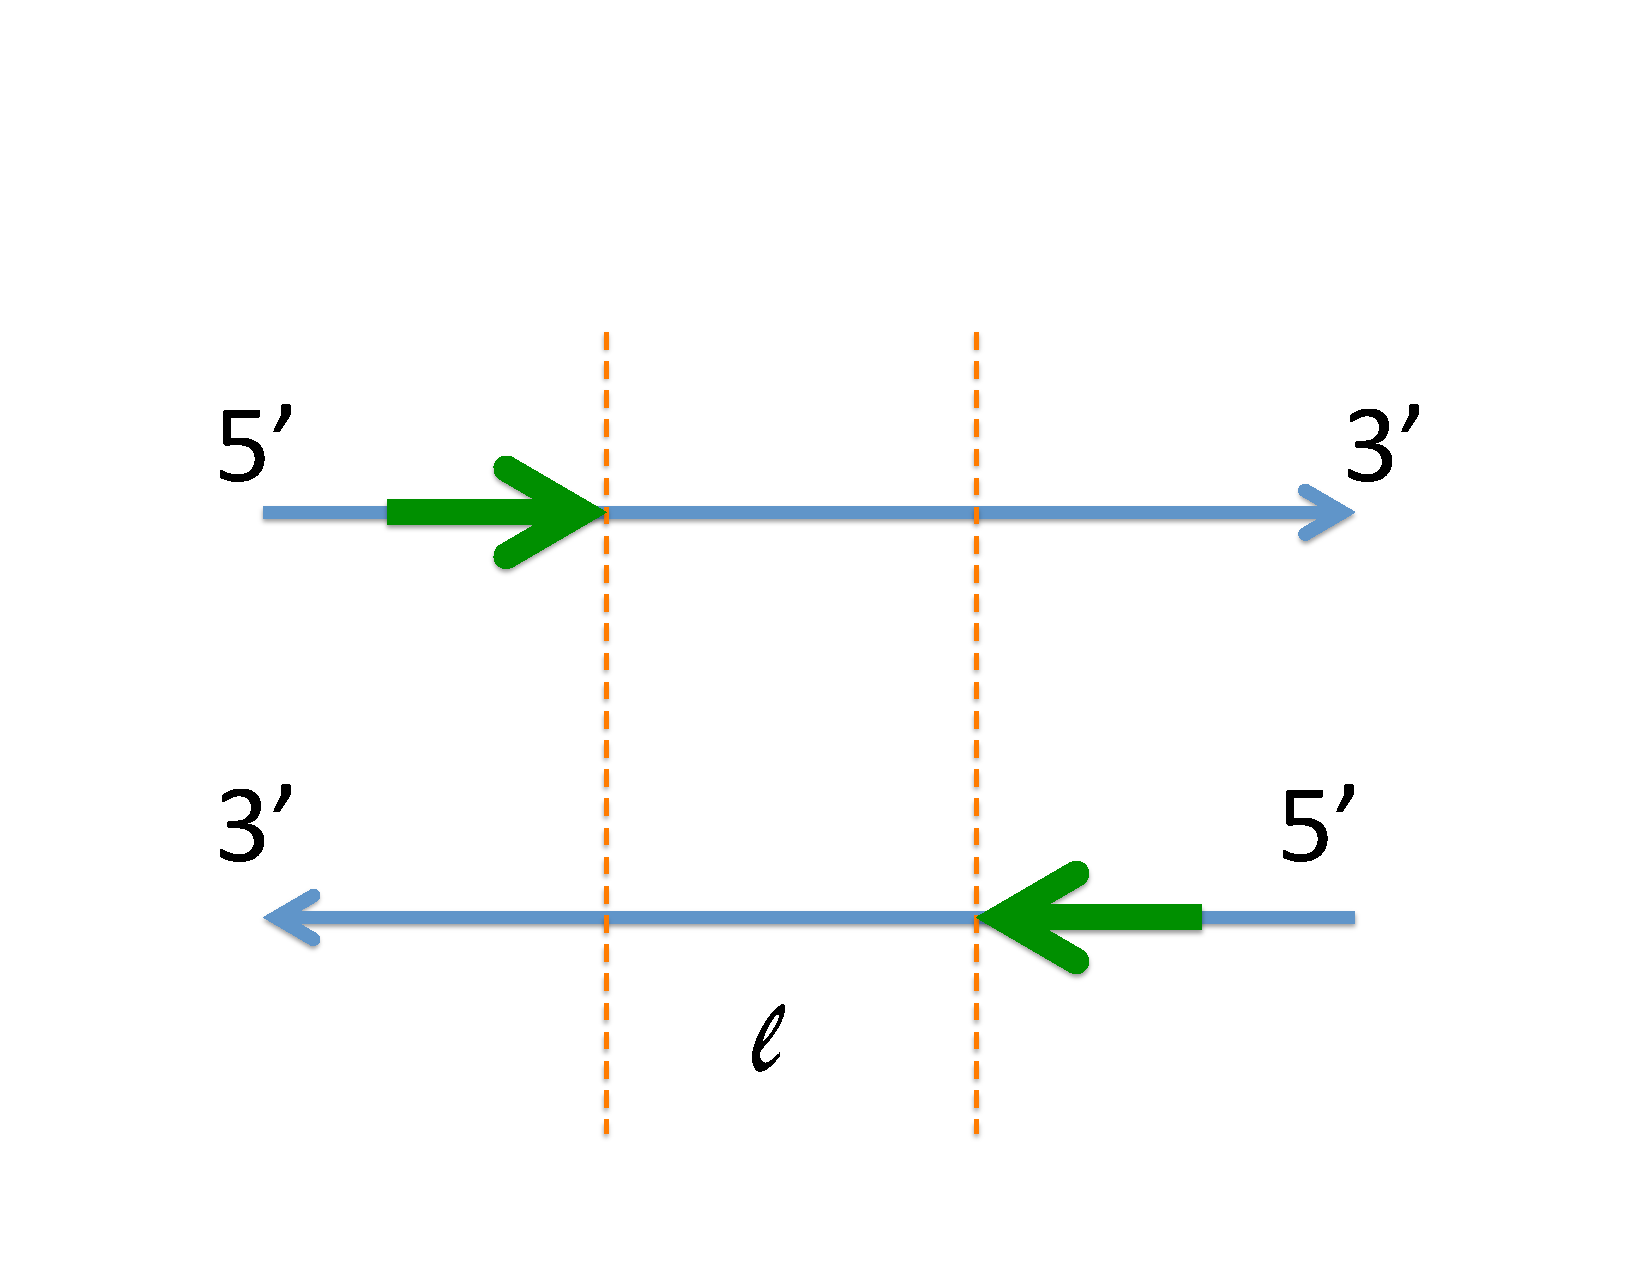
\includegraphics[width=6in]{./bioinformatics/pics/bowtie_example}
\caption{An example of Bowtie, as it tries to align a subsequence in a DNA sequence with another subsequence in another DNA sequence.}
\label{fig:BowtieExample}
\end{figure}

An example of DNA sequences being read by {\tt Bowtie} is shown in Figure \ref{fig:BowtieExample}. \\


Separate the reads into different classes, especially for genomes with lots of single nucleotide polymorphism (SNPS) $\rightarrow$ lots of inversion that need to be sorted.













%%%%%%%%%%%%%%%%%%%%%%%%%%%%%%%%%%%%%%%%%%%%%%
\section{SAM File Format}
\label{sec:SAMFileFormat}

The second field of the {\tt SAM} file format indicates various information about the alignment and pairing. It indicates the call of a proper read, or align read. The majority of the reads don't map well because we are mapping only to the smallest chromosome of the species. The {\it Neurospora crassa} species has 7 chromosomes\dots\ Without paired reads, the numbers are different. \\

Some calculations to determine such information is demonstrated as follows: \vspace{-0.3cm}
\begin{enumerate} \itemsep -4pt
\item 77 = 64 + 8 + 4 + 1
\item 141 = 128 + 8 + 4 + 1
\item 163 = 128 + 32 + 2 + 1. Properly aligned.
\item 83 = 64 + 16 + 2 + 1
\item 99 = 64 + 32 + 2+ 1
\end{enumerate}

Convert {\tt SAM} files to {\tt BAM} files, which are faster to read. {\tt SAM} files are written according to when they (i.e., the subsequences) are found/read; that is, they are written as the subsequences are found. On the other hand, the {\tt BAM} files can be sorted according to their coordinates of the beginning (and, hence, the end) of the subsequences; {\it verify this!!!}. These {\tt BAM} files are sorted from left to right. For scientific/experimental control, show that the {\tt SAM} file that is re-converted from {\tt BAM} is sorted; that is, check that the recovered {\tt SAM}-to-{\tt BAM}-to-{\tt SAM} file is sorted. \\

Use {\tt Fasta} (.fasta) and {\tt .fa} files. Sorted {\tt SAM} files have no header. Reads are mapped and primed in ordered fashion, without the header. They can't be displayed on their own, and require another file for its contents to be displayed. Specifically, an index {\tt BAM} file needs to be provided with the sorted {\tt BAM} file. When the data is viewed (with the script {\tt ./igv.sh}), it shows valleys and peaks. The peaks indicate a good probability of having contigs. The valleys indicate a good probability of not having connected contigs (or a high probability of not having a connection is high); use make pair to ``weaken connection''??? \dots\ The colored regions are repeated subsequences that indicate polymorphism. \\

Grab???, scrub???, clone, and sequence DNA. Extract the DNA, build its library, and sequence without cloning. Structure DNA $\longleftrightarrow$ sequence, making the library and PCR for sequencing bad. Base-call qualities are rejected. There exists different levels of PCR, or different uses of PCR in this process. When errors are present in the displayed DNA sequence, it could be because something was wrong with the PCR or there were problems during sequencing. The centropid (or centromere)\dots\ exists in mitochondrial DNA (or mtDNA)? It repeats regularly. \\

There exists two {\tt Bowtie} programs. {\tt Bowtie} is different from {\tt Bowtie 2}, and they require different input file formats. Hence, {\tt Bowtie 2} files are for {\tt Bowtie 2} only. \#1 mates indicate forward reads, and \#2 mates indicate reverse reads. Concordantly, read1 and read2 must be mapped, as expected. Else, if they are not mapped, they cannot be used for genome assembly [discordantly]. \\

{\tt Bowtie 2} has two mapping modes, which are different to separate. They are end-to-end mapping and local mapping. \\

For the end-to-end mapping mode of {\tt Bowtie 2}: \vspace{-0.3cm}
\begin{enumerate} \itemsep -4pt
\item Very fast global mapping
\item Fast global mapping
\item Sensitive global mapping
\item Very sensitive global mapping
\end{enumerate}

For the local mapping mode of {\tt Bowtie 2}: \vspace{-0.3cm}
\begin{enumerate} \itemsep -4pt
\item Very fast local mapping
\item Fast local mapping
\item Sensitive local mapping
\item Very sensitive local mapping
\end{enumerate}

Control the number to change the sensitivity, so that diversions can be dealt with. The computational time taken (i.e., performance of the procedure/software) changes with respect to sensitivity. That is, the performance of the {\tt Bowtie 2} algorithm is proportional to sensitivity. As sensitivity increases, the time taken (or computational complexity, or performance) increases. \\

Genome assembly needs to be carried out, since we fragment DNA and now we have to assemble it. Copy the mapped files and look at the regions between n3m1 and n3m100, and display the results. Show how the {\tt -n} and {\tt -m} parameters affect mapping; that is, genomic mapping is affected by the parameters. Thus far, we are mapping DNA reads. \\

When mooing RNA reads, things are more different. RNA has lots of contigs, which form a library. Genomic maps are generated from transcriptome mapping, which has its equivalent genome (and, thus, its own contigs). They depend on contigs, and are products of the genomic assembly process. Here, we are constructing the DNA sequence from the contigs. \\

Reads exist in eons. They map to introns/exons. However, at the boundaries of introns and exons, they do not follow rules. Therefore, we cannot use {\tt Bowtie} to resolve the mapping. Consequently, we need to carry out transcriptome mapping. Genomic assembly: randomly assemble 1 read with another read that overlaps it at the edges. This construction of contigs using contiguous DNA sequences builds up the genome. Again, look for overlaps in the DNA sequences to assemble the genome. Instead of reads, programs grab a k-mer (i.e., n-tuple and n-gram Nucleic acid sequence, amino acid sequence, or polymer)??? \dots\ For a k-mer of 13, it refers to a k-mer of 13 bases. \\

Our reads are of 50 bases. {\tt Velvet} is a Blue Gene graft-based assembler. \\

Do not print graphs with bases, because they are huge. Assemble fractions of chromosomes (linkage to Group VII of the {\it Neurospora species}. \\


Suggestions for 



























